\section{Introduzione}

\subsection{Glossario}
In questo documento sono state segnate con il pedice "g" tutte le parole che, secondo noi, necessitano di una spiegazione ulteriore per evitare
eventuali ambiguità o incomprensioni.

La spiegazione di questi termini la si può trovare nel documento di \textit{Glossario}.

\subsection{Scopo del documento}
Il documento \textit{Specifica Tecnica} ha lo scopo di descrivere i componenti utilizzati e le scelte progettuali fatte per la realizzazione del prodotto.

Dopo aver fornito un elenco descrittivo dei componenti verranno spiegati nel dettaglio, utilizzando l'ausilio degli schemi UML, i seguenti punti di interesse: 
\begin{itemize}
	\item Design pattern architetturale determinato dalle tecnologie adottate;
	\item Architettura logica (connessioni e interazioni tra componenti);
	\item Architettura di deployment (l’allocazione di componenti nel sistema in esecuzione);
	\item Idiomi, pattern di livello più basso che architetturale;
	\item Ogni altro aspetto progettuale che valorizza o caratterizza il design utilizzato.
\end{itemize}

\subsection{Suggerimenti per la comprensione del documento}
Per comprendere al meglio l'architettura utilizzata è importante comprendere in primo luogo il design pattern
architetturale derterminato dalle tecnologie adottate in quanto gran parte delle scelte fatte si basano su di esso.

\textbf{Si suggerisce quindi di leggere la sezione} \ref{design Redux} \textbf{riguardante il design pattern architetturale determinato 
dalle tecnologie adottate prima di proseguire con le successive}.

\section{Descrizione dell'architettura}
\subsection{Elenco dei componenti}
\begin{itemize}
	\item \textbf{\large Slices}:
		\begin{itemize}
			\item \textbf{CartSlice}: componente che permette la gestione dello stato che contiene i dati riguardanti il carrello;
			\item \textbf{ProductsSlice}: componente che permette la gestione dello stato che contiene i dati riguardanti i prodotti 
			presenti all'interno dell'ambiente 3D.
			\item \textbf{PlayerSlice}:
			\item \textbf{RayCasterSlice}:
			\item \textbf{DecorationSlice}: 
			\item \textbf{SidebarSlice}:
		\end{itemize}
	\item \textbf{\large Initial states}:
		\begin{itemize}
			\item \textbf{CartInitialState}:
			\item \textbf{ProductsInitialState}:
			\item \textbf{PlayerInitialState}:
			\item \textbf{RayCasterInitialState}:
			\item \textbf{DecorationInitialState}:
			\item \textbf{SidebarInitialState}:
		\end{itemize}
		\item \textbf{\large Actions}:
		\begin{itemize}
			\item \textbf{sidebar.toggleSidebarIsOpen}:
			\item \textbf{rayCaster.setLastProductPointed}:
			\item \textbf{rayCaster.toggleRayCasterEnabled}:
			\item \textbf{cart.addItems}:
			\item \textbf{cart.removeItem}:
			\item \textbf{cart.removeAll}: 
		\end{itemize}
		\item \textbf{\large Model components}:
		\begin{itemize}
			\item \textbf{Coordinate}:
			\item \textbf{Camera}:
			\item \textbf{Octree}:
			\item \textbf{Vector3}:
			\item \textbf{Capsule}:
			\item \textbf{Player}:
			\item \textbf{CartItem}:
		\end{itemize}
		\item \textbf{\large UI React components}:
		\begin{itemize}
			\item \textbf{UI}:
			\item \textbf{Crosshair}:
			\item \textbf{Cart}:
			\item \textbf{PlayerPosition}:
			\item \textbf{CartItem}:
			\item \textbf{ProductUI}:
			\item \textbf{ProductInteractionPrompt}:
			\item \textbf{Sidebar}:
			\item \textbf{ColorSelector}:
			\item \textbf{SelectColorItem}:
			\item \textbf{ProductDetails}:
		\end{itemize}
		\item \textbf{\large 3D React components}:
		\begin{itemize}
			\item \textbf{Canvas}:
			\item \textbf{Scene}:
			\item \textbf{PointerLock}:
			\item \textbf{Environment}:
			\item \textbf{Map}:
			\item \textbf{Player}:
			\item \textbf{Lights}:
			\item \textbf{Models}:
			\item \textbf{Decorations}:
			\item \textbf{RayCaster}:
		\end{itemize}
\end{itemize}
\subsection{Design pattern architetturale determinato dalle tecnologie adottate}
\label{design Redux}

\subsubsection{Redux-Toolkit}
I componenti che costituiscono l'architettura utilizzata seguono il pattern offerto dalla libreria Redux-Toolkit.

Redux-Toolkit è pensato per integrarsi con React e il principale vantaggio che offre è quello di poter gestire i dati condivisi tra 
i componenti React in modo centralizzato semplificando la gestione dello stato globale dell'applicazione 
(in alternativa ogni componente React dovrebbe passare il proprio stato tramite props ai suoi diretti discendenti).
\\\\
I componenti che formano l'architettura di Redux-Toolkit sono:
\begin{itemize}
	\item \textbf{Store}: componente che contiene lo stato globale dell'applicazione.
	
	All'avvio dell'applicazione viene configurato utilizzando RootReducer e i componenti che utilizzano lo stato globale fanno il subscribe allo \textit{store}
	in modo da venire renderizzati ogni volta che un dato di interesse cambia valore.
	Questo modo di operare può essere visto come un pattern \textit{Observer} in cui lo \textit{store} è il \textit{Subject} e gli \textit{Observers} sono i componenti React che hanno fatto 
	il subscribe allo \textit{store};
	\item \textbf{RootReducer}: componente utilizzato per configurare lo store combinando più slice;
	\item \textbf{Slice}: componente che contiene un proprio stato che rappresenta una porzione dello stato globale dell'applicazione, i \textit{reducer}
	che operano sullo stato e i \textit{selector} per consentire ai suoi client il reperimento dei dati. 

	Per definire una \textit{slice} è buona norma raggruppare i dati in modo che siano legati da un sottoinsieme di funzionalità offerte dal sistema che lavorano 
	su dati comuni;  
	\item \textbf{Reducer}: componente che riceve come parametri uno stato iniziale (\textit{InitialState}) e una \textit{action} (composta da un type e un payload) e restituisce 
	lo stato dopo aver operato sui dati. 
	
	React-Toolkit gestisce le chiamate ai \textit{reducer} quindi i dispatch delle \textit{action} avvengono
	specificando solamente l'oggetto che rappresenta il payload; 
	\item \textbf{Actions}: oggetto composto da un type e da un payload di cui viene effettuato il dispatch quando opportuno. 
	
	Il payload è un oggetto che contiene i dati da passare al \textit{reducer} che catturerà l'\textit{action};
	\item \textbf{InitialState}: componente che contiene i dati di una \textit{slice} su cui essa opera. 
	
	Importante precisare che Redux-Toolkit utilizzando 
	la libreria immer gestisce anche l'immutabilità dei dati in modo che i reducer restituiscano delle copie dello stato in modo che esso non possa 
	venire modificato dall'esterno e utilizzato in modo improrio.
	
	L'unico modo per modificare i dati dello stato globale è quindi con il dispatch di un'\textit{action};
	\item \textbf{Selector}: funzione che prende lo stato corrente di una \textit{slice} come argomento e ritorna un sottoinsieme specifico
	del suo stato. In altre parole, un \textit{selector} consente di 'selezionare' una parte specifica dello stato
	in modo da poterla utilizzare in modo isolato all'interno di un componente React.
\end{itemize}

\subsubsection{React-three-fiber}
Questa libreria fornisce un 'punto d'incontro' tra React (libreria javascript per la creazione di interfacce utente) e Three.js (libreria usata per
la modellazione dell'ambiente 3D) semplificando la creazione dei componenti da inserire all'interno dell'ambiente 3D.

React-three-fiber rende la scrittura del codice dichiarativa creando dei componenti React 'preconfezionati' che rappresentano i componenti 3D.
Questi componenti sono personalizzabili modificandone le caratteristiche tramite le props di React.

Un esempio è il componente \textit{Canvas} che fornisce con un'unica dichiarazione la \textit{scene} e la \textit{camera} con una configurazione standard 
adatta alla maggior parte dei casi di utilizzo. Per inserire i componenti all'interno dell'ambiente è sufficiente dichiararli come figli del 
componente \textit{scene}.
\subsection{Architettura logica}
Per facilitare la lettura dei diagrammi delle classi è stato scelto di organizzarli per feature in modo che ogni diagramma 
rappresenti i componenti che permettono l'implementazione di funzionalita' specifiche.
Sono presenti dei diagrammi che non seguono questa convenzione che sono utili per avere una visione generale sulle dipendenze
di alcuni componenti.
\\\\
I diagrammi prodotti che rappresentano funzionalità specifiche sono:
\begin{itemize}
	\item \textbf{CartFeaturesDiagram:} include i componenti che svolgono le funzioni riguardanti il carrello;
	\item \textbf{PlayerFeaturesDiagram:} include i componenti che svolgono le funzioni riguardanti le interazioni dell'utente con 
	l'ambiente 3D;
	\item \textbf{ProductSidebarFeaturesDiagram:} include i componenti che svolgono le funzioni riguardanti la side-bar;
	\item \textbf{InterfaceFeaturesDiagram:} include i componenti necessari per il corretto aggiornamento dell'interfaccia utente;
\end{itemize}
I diagrammi prodotti che forniscono una visione generale delle dipendenze tra componenti sono:
\begin{itemize}
	\item \textbf{StoreDiagram:} include lo \textit{store};
	\item \textbf{ReactComponentsHierarchy:} include i componenti React che rappresentano l'interfaccia utente e la scena 3D.
\end{itemize}

\subsubsection{CartFeaturesDiagram}
\label{CartFeaturesDiagram}
\begin{figure}[H]
	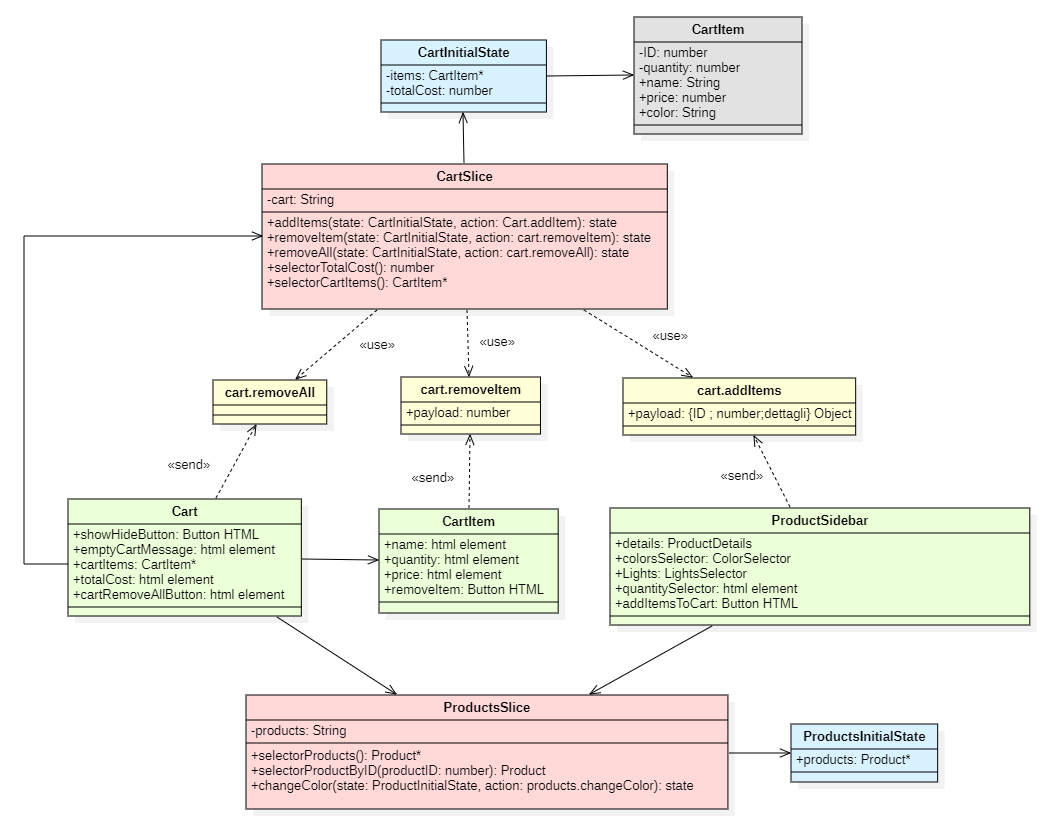
\includegraphics[width=1\textwidth, keepaspectratio]{./res/images/cart_features.PNG}
	\caption[UML delle classi CartFeaturesDiagram]{
	UML delle classi CartFeaturesDiagram.
	\\
	\textbf{Legenda}: 
	[\textit{Slices}: rosso] -
	[\textit{Actions}: giallo] -
	[\textit{Model classes}: grigio] -
	[\textit{Initial states}: azzurro] -
	[\textit{UI React components}: verde]}
\end{figure}

\paragraph*{Descrizione del diagramma:}
CartFeaturesDiagram contiene i componenti coinvolti nelle interazioni con il carrello.
\begin{itemize}
		\item \textbf{CartSlice}
		\begin{itemize}
			\item \textit{Connessioni}:
			\item \textit{Interazioni}:
		\end{itemize}
		\item \textbf{ProductsSlice}
		\begin{itemize}
			\item \textit{Connessioni}:
			\item \textit{Interazioni}:
		\end{itemize} 
		\item \textbf{CartInitialState}
		\begin{itemize}
			\item \textit{Connessioni}:
			\item \textit{Interazioni}:
		\end{itemize} 
		\item \textbf{ProductsInitialState}
		\begin{itemize}
			\item \textit{Connessioni}:
			\item \textit{Interazioni}:
		\end{itemize} 
		\item \textbf{cart.removeAll}
		\begin{itemize}
			\item \textit{Connessioni}:
			\item \textit{Interazioni}:
		\end{itemize} 
		\item \textbf{cart.removeItem}
		\begin{itemize}
			\item \textit{Connessioni}:
			\item \textit{Interazioni}:
		\end{itemize} 
		\item \textbf{cart.addItems}
		\begin{itemize}
			\item \textit{Connessioni}:
			\item \textit{Interazioni}:
		\end{itemize} 	
		\item \textbf{CartItem}
		\begin{itemize}
			\item \textit{Connessioni}:
			\item \textit{Interazioni}:
		\end{itemize} 
		\item \textbf{Cart}
		\begin{itemize}
			\item \textit{Connessioni}:
			\item \textit{Interazioni}:
		\end{itemize} 
		\item \textbf{CartItem}
		\begin{itemize}
			\item \textit{Connessioni}:
			\item \textit{Interazioni}:
		\end{itemize} 
		\item \textbf{ProductSidebar}
		\begin{itemize}
			\item \textit{Connessioni}:
			\item \textit{Interazioni}:
		\end{itemize} 
	\end{itemize}
	


\subsubsection{PlayerFeaturesDiagram}


\subsubsection{SidebarFeaturesDiagram}


\subsubsection{InterfaceFeaturesDiagram}


\subsubsection{StoreDiagram}


\subsection{Architettura di deployment}
\subsection{Idiomi e pattern di livello più basso}
\subsection{Altri aspetti di design}
























\subsection{Riferimenti}
\subsubsection{Riferimenti normativi}
\begin{itemize}
\item Capitolato d’appalto C6: \url{https://www.math.unipd.it/~tullio/IS-1/2022/Progetto/C6.pdf};
\item \textit{Norme di Progetto};
\item \textit{Verbale esterno 17/11/22};
\item \textit{Verbale interno 01/12/22};
\item \textit{Verbale interno 07/12/22};
\item \textit{Verbale esterno 11/01/23};
\item \textit{Verbale esterno 18/01/23};
\item \textit{Verbale esterno 17/02/23};
\item \textit{Verbale interno 24/02/23}.
\end{itemize}

\subsubsection{Riferimenti informativi}
\begin{itemize}
\item Presentazione del capitolato: \url{https://www.math.unipd.it/~tullio/IS-1/2022/Progetto/C6.pdf};

\item Three.Js - Riferimenti:
\begin{itemize}
\item Fondamenti di Three.js: \url{https://threejs.org/manual/#en/fundamentals};
\item Documentazione Three.js: \url{https://threejs.org/docs/index.html#manual/en/introduction/Creating-a-scene};
\item Repository\textsubscript{g} informativa Three.js: \url{https://github.com/mrdoob/three.js/}.
\end{itemize} 
\end{itemize} 